% This is "sig-alternate.tex" V2.1 April 2013
% This file should be compiled with V2.5 of "sig-alternate.cls" May 2012
%
% This example file demonstrates the use of the 'sig-alternate.cls'
% V2.5 LaTeX2e document class file. It is for those submitting
% articles to ACM Conference Proceedings WHO DO NOT WISH TO
% STRICTLY ADHERE TO THE SIGS (PUBS-BOARD-ENDORSED) STYLE.
% The 'sig-alternate.cls' file will produce a similar-looking,
% albeit, 'tighter' paper resulting in, invariably, fewer pages.
%
% ----------------------------------------------------------------------------------------------------------------
% This .tex file (and associated .cls V2.5) produces:
%       1) The Permission Statement
%       2) The Conference (location) Info information
%       3) The Copyright Line with ACM data
%       4) NO page numbers
%
% as against the acm_proc_article-sp.cls file which
% DOES NOT produce 1) thru' 3) above.
%
% Using 'sig-alternate.cls' you have control, however, from within
% the source .tex file, over both the CopyrightYear
% (defaulted to 200X) and the ACM Copyright Data
% (defaulted to X-XXXXX-XX-X/XX/XX).
% e.g.
% \CopyrightYear{2007} will cause 2007 to appear in the copyright line.
% \crdata{0-12345-67-8/90/12} will cause 0-12345-67-8/90/12 to appear in the copyright line.
%
% ---------------------------------------------------------------------------------------------------------------
% This .tex source is an example which *does* use
% the .bib file (from which the .bbl file % is produced).
% REMEMBER HOWEVER: After having produced the .bbl file,
% and prior to final submission, you *NEED* to 'insert'
% your .bbl file into your source .tex file so as to provide
% ONE 'self-contained' source file.
%
% ================= IF YOU HAVE QUESTIONS =======================
% Questions regarding the SIGS styles, SIGS policies and
% procedures, Conferences etc. should be sent to
% Adrienne Griscti (griscti@acm.org)
%
% Technical questions _only_ to
% Gerald Murray (murray@hq.acm.org)
% ===============================================================
%
% For tracking purposes - this is V2.0 - May 2012

\documentclass{sig-alternate}

\begin{document}

% Copyright
\setcopyright{acmcopyright}
%\setcopyright{acmlicensed}
%\setcopyright{rightsretained}
%\setcopyright{usgov}
%\setcopyright{usgovmixed}
%\setcopyright{cagov}
%\setcopyright{cagovmixed}


% DOI
\doi{10.475/123_4}

% ISBN
\isbn{123-4567-24-567/08/06}

%Conference
\conferenceinfo{CS519 Sensemaking in Soft. Eng. '16}{January 4--March 18, 2016, Corvallis, OR, USA}

\acmPrice{\$15.00}

%
% --- Author Metadata here ---
\conferenceinfo{CS519 Sensemaking in Soft. Eng.}{'16 Corvallis, Oregon USA}
%\CopyrightYear{2007} % Allows default copyright year (20XX) to be over-ridden - IF NEED BE.
%\crdata{0-12345-67-8/90/01}  % Allows default copyright data (0-89791-88-6/97/05) to be over-ridden - IF NEED BE.
% --- End of Author Metadata ---

\title{A Sensemaking Approach to Continuous Integration}
%
% You need the command \numberofauthors to handle the 'placement
% and alignment' of the authors beneath the title.
%
% For aesthetic reasons, we recommend 'three authors at a time'
% i.e. three 'name/affiliation blocks' be placed beneath the title.
%
% NOTE: You are NOT restricted in how many 'rows' of
% "name/affiliations" may appear. We just ask that you restrict
% the number of 'columns' to three.
%
% Because of the available 'opening page real-estate'
% we ask you to refrain from putting more than six authors
% (two rows with three columns) beneath the article title.
% More than six makes the first-page appear very cluttered indeed.
%
% Use the \alignauthor commands to handle the names
% and affiliations for an 'aesthetic maximum' of six authors.
% Add names, affiliations, addresses for
% the seventh etc. author(s) as the argument for the
% \additionalauthors command.
% These 'additional authors' will be output/set for you
% without further effort on your part as the last section in
% the body of your article BEFORE References or any Appendices.

\numberofauthors{2} %  in this sample file, there are a *total*
% of EIGHT authors. SIX appear on the 'first-page' (for formatting
% reasons) and the remaining two appear in the \additionalauthors section.
%
\author{
% You can go ahead and credit any number of authors here,
% e.g. one 'row of three' or two rows (consisting of one row of three
% and a second row of one, two or three).
%
% The command \alignauthor (no curly braces needed) should
% precede each author name, affiliation/snail-mail address and
% e-mail address. Additionally, tag each line of
% affiliation/address with \affaddr, and tag the
% e-mail address with \email.
%
% 1st. author
\alignauthor
Nicholas Nelson\\
       \affaddr{Oregon State University}\\
       \affaddr{Corvallis, Oregon}\\
       \email{nelsonni@oregonstate.edu}
% 2nd. author
\alignauthor
Charles Hill\\
       \affaddr{Oregon State University}\\
       \affaddr{Corvallis, Oregon}\\
       \email{hillc@oregonstate.edu}
}
% Just remember to make sure that the TOTAL number of authors
% is the number that will appear on the first page PLUS the
% number that will appear in the \additionalauthors section.

% shortcut macros for Study Participants
\newcommand{\michael}{P1 }
\newcommand{\sruti}{P2 }
\newcommand{\caius}{P3 }
\newcommand{\srutitwo}{P4 }
\newcommand{\david}{P5 }
\newcommand{\cpg}{P6 }

\maketitle
\begin{abstract}
\end{abstract}
%%%%The problem
Continuous integration is gaining traction as part of the software development lifecycle, but little work has been done to understand how its use affects developers.
%%%%Why it matters
This is a problem if we want to be able to support developers in their use of continuous integration: if we don't understand how people use it, we can't improve it.
%%%%Here's what we did
 In this paper, we investigate the way developers make sense of their continuous integration system results in the context of their development cycle. To find out how software developers make sense of their continuous integration tool and its output, we interviewed professionals about their experiences with continuous integration.
%%%%Here's how it'll change the world :O
We present modifications to the sensemaking model that better reflect developers' use of continuous integration.
\smallskip

\begin{CCSXML}
<ccs2012>
 <concept>
  <concept_id>10010520.10010553.10010562</concept_id>
  <concept_desc>Computer systems organization~Embedded systems</concept_desc>
  <concept_significance>500</concept_significance>
 </concept>
 <concept>
  <concept_id>10010520.10010575.10010755</concept_id>
  <concept_desc>Computer systems organization~Redundancy</concept_desc>
  <concept_significance>300</concept_significance>
 </concept>
 <concept>
  <concept_id>10010520.10010553.10010554</concept_id>
  <concept_desc>Computer systems organization~Robotics</concept_desc>
  <concept_significance>100</concept_significance>
 </concept>
 <concept>
  <concept_id>10003033.10003083.10003095</concept_id>
  <concept_desc>Networks~Network reliability</concept_desc>
  <concept_significance>100</concept_significance>
 </concept>
</ccs2012>  
\end{CCSXML}

% We no longer use \terms command
%\terms{Theory}

\keywords{Continuous Integration; Sensemaking; Human-Computer Interactions; Software Engineering}

\section{Introduction}
Agile development models have replaced traditional development models (such as Waterfall Method) in a significant portion of the professional software development industry. Continuous integration is an optional part of agile development, currently practiced by many large companies such as Facebook, Google, Netflix, and LinkedIn.

Continous Integration describes a set of software engineering practices that speed up the delivery of software by automating the integration and build steps of the software development cycle. It emerged in the Extreme Programming (XP) community, with Kent Beck and Ron Jeffries writing about agile development models and continuous integration while on the Chrysler Comprehensive Compensation System project in 1998\cite{beck:extreme_programming}\cite{beck:agile_manifesto}.

Martin Fowler further described the concept of continuous integration in 2006, by defining \textit{continuous integration} as:
\begin{quote}
Continuous Integration is a software development practice where members of a team integrate their work frequently, usually each person integrates at least daily -- leading to multiple integrations per day. Each integration is verified by an automated build (including test) to detect errors as quickly as possible. Many teams find that this approach leads to significantly reduced integration problems and allows a team to develop cohesive software more rapidly.\cite{fowler:continuous}
\end{quote}

Little research has been done, though, to understand its effect on developers. In order to have an informed discussion about the actualized benefits and realized detriments inherent to continuous integration, we must first understanding the motivations, methods, and usage associated with it.

Previous studies on continuous integration have focused on the operational and integrational aspects of using continuous integration as part of an agile software development process\cite{miller:hundreddays}\cite{olsson:climbingstairway}, use within open source projects\cite{deshpande:ci_opensource}, or as a foil for comparison between traditional and agile development models\cite{staahl:modelingdiffs}. There are no studies that examine the effects continuous integration has on sensemaking and comprehension for software development tasks.

In this paper we attempt to evaluate whether Peter Pirolli and Stuart Card's \textit{notional model of sensemaking}\cite{pirolli:sensemaking} can be applied to the use of continuous integration, whether the use of continuous integration in software development alters the previously observed model, and whether the use of continuous integration achieves the goals that professional software developers strive for when integrating continuous integration into their development processes.

Development tools are only helpful when used by software developers, therefore the adoption of these tools is critical for their success. Tool developers must understand the needs and usage patterns of their users

Learning how developers' comprehend and evaluate their software development processes when continuous integration tools and processes are employed will allow tool designers to better target perspective users.

This study is an attempt to learn more about software developers' sensemaking associated with continuous integration. To that end, we look for answers to the following research questions:
\begin{itemize}
\item RQ1: Does Pirolli's Sensemaking Model apply to Continuous Integration?
\item RQ2: Does Continuous Integration alter programmers' sensemaking behavior?
\item RQ3: Does the use of continuous integration aid developers in making sense of their software development cycles?

\end{itemize}
%%%%%%

\section{Background and Related Work}

the usage of continuous integration has primarily focused upon the operational aspects of continuous integration as it relates to software development processes \cite{miller:hundreddays}\cite{olsson:climbingstairway}.

\section{Methodology} \label{method}

To answer our research questions, we conducted semi-structured interviews, wherein we asked a list of pre-set questions and inquired further with follow-up questions to learn more about each participant. \\

\begin{table*}
\label{table:codeset}
\centering
\caption{Codeset}
\begin{tabular}[b]{ | l | l | p{5.5cm} | p{6.5cm} | }
	\hline
	\rowcolor{black!20!} Code & Code Name & Description & Rules / Examples \\ \hline
	EDS & External Data Sources & Raw evidence in mostly standard consumable formats (text). & Existing external artifacts associated with software development (i.e. source code, test suites, databases, raw data, servers, etc.) \\ \hline
	SHOE & Shoebox & Much smaller subset of that external data that is relevant for processing. & Modifications to source code or testing artifacts (i.e. commits, changesets, updates) \\ \hline
	EVID & Evidence File & Snippets extracted from items in the shoebox. & Integration, compilation, and building actions related to modification and changes \\ \hline
	SCHM & Schema & Re-representation or organized marshalling of the information so that it can be used more easily to draw conclusions. & Results of integration, compilation, building, and updating (i.e. build reports, metrics, status dashboards, etc.) \\ \hline
	HYPO & Hypothesis & Tentative representation of those conclusions with supporting arguments. & Assumptions regarding integration, compilation, and builds, or conclusions drawn from the results of such actions \\ \hline
	PRES & Presentation & The final work product which is suited for communication. & Final software product, successfully build product, or deployment to customers \\ \hline
\end{tabular}
\end{table*}

We interviewed 6 participants, each of whom had at least three years software development experience. Participant information is detailed in table \ref{table:participant}. Participant roles in the software development process varied. For instance, one participant (\cpg) was a founding member of a startup who managed the development team, while another participant (\david) worked for an international software company. The average experience level with software development was **x years, with a maximum of **x. All participants were required to have at least some experience with continuous integration; no minimum level was required.

\begin{table}
\centering
\label{table:participant}
\caption{Participant Information}
\begin{tabular}{ | >{\centering\arraybackslash}p{.25\columnwidth} | >{\centering\arraybackslash}p{.25\columnwidth} | >{\centering\arraybackslash}p{.25\columnwidth} | }\hline
	\rowcolor{black!20!}Participant number & Development experience & Continuous Integration Experience \\ \hline
	\michael & 1 & 1 \\ \hline
	\sruti & 2 & 2 \\ \hline
	\caius & 3 & 3 \\ \hline
	\srutitwo & 4 & 4 \\ \hline
	\david & 5 & 5 \\ \hline
	\cpg & 6 & 6 \\ \hline
\end{tabular}
\end{table}

Our semi-structured interviews took place in person in a conference room at an engineering center. The exception was \cpg, who was interviewed at their place of work. Interviews lasted an average of 30 minutes, with a minimum of 8 minutes. All interviews were audio recorded with permission from participants.  Interviews began with demographic questions: participant development experience, and experience with continuous integration. We also asked a thematic question:

\smallskip
\textit{"Tell me about the last time you used continuous integration"}


For the rest of the interview, participants referred back to that experience with continuous integration. Here are some sample questions we used to get information about participants' sensemaking behavior:
\begin{itemize}  
	\item What tasks prompt you to interact with your current CI tools?
	\item What outside information do you use to evaluate the information provided by your CI solution?
	\item What types of information from your CI solution do you find relevant to you? 
\end{itemize}

\subsection{Analysis}
After transcribing the interviews, we analyzed them by using a code set based on Pirolli and Card's sensemaking model \cite{pirolli:sensemaking}. We operationalized the steps in the sensemaking model as described in Table \ref{table:codeset}. Participant transcripts were analyzed at the sentence level. We limited codes to one count of each code per sentence; if a sentence mentioned EDS twice, for example, only one instance was coded. Multiple code types were allowed for each sentence. We coded 20.37\% of participant data and reached 80.8\% agreement, measured using the Jaccard index. After that, participant data was coded independently.

\section{Results}

\subsection{RQ1:  Does Pirolli's Sensemaking Model apply to Continuous Integration?}
\begin{figure*}
\centering
\frame{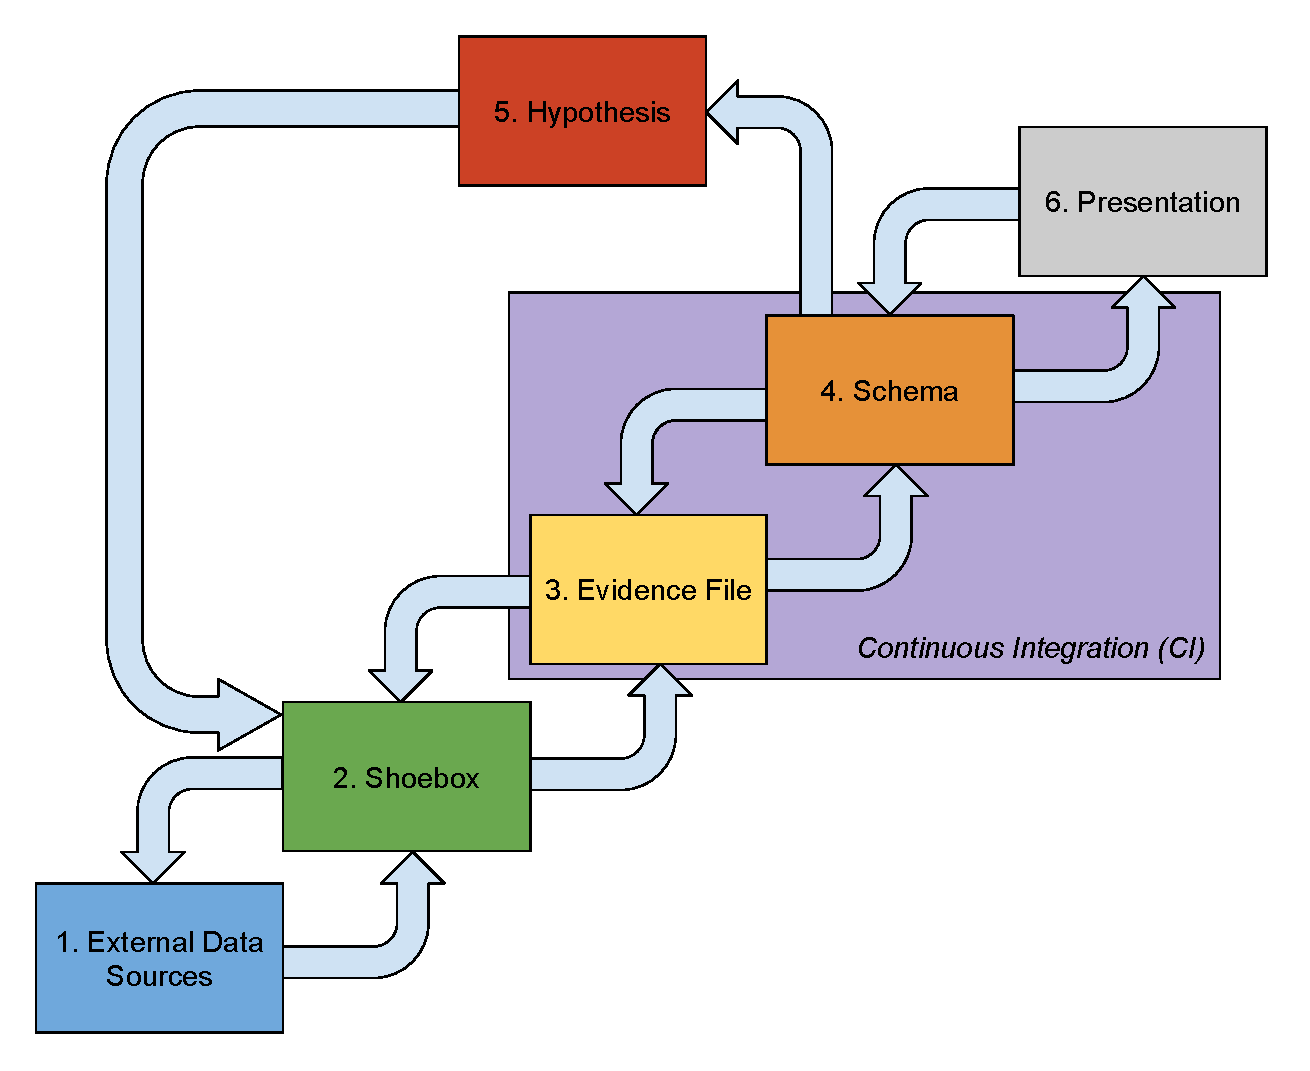
\includegraphics[height=9cm, width=0.6\textwidth]{sensemaking_model}}
\caption{A sample black and white graphic
that has been resized with the \texttt{includegraphics} command.}
\end{figure*}

To answer this question, we coded participant interviews as described in the Methodology (Section \ref{method}).


\subsection{RQ2: Does Continuous Integration alter the programmer's sensemaking behavior?}
\begin{table}
	\centering
	\caption{Code Results}
	\label{table:coderesults}
	\begin{tabular}{ | >{\centering\arraybackslash}p{.25\columnwidth} | m{0.4cm} | l | l | l | l | l | l | }
		\hline
		\rowcolor{black!20!}Code & P1 & P2 & P3 & P4 & P5 & P6 & Total \\ \hline
		EDS & 4 & 12 & 12 & 14 & 12 & 8 & 72 \\ \hline
		SHOE & 3 & 5 & 10 & 10 & 19 & 2 & 59 \\ \hline
		EVID & 0 & 6 & 11 & 17 & 13 & 11 & 67 \\ \hline
		SCHM & 4 & 15 & 17 & 13 & 22 & 18 & 90 \\ \hline
		HYPO & 2 & 0 & 2 & 4 & 7 & 7 & 27 \\ \hline
		PRES & 0 & 0 & 0 & 0 & 1 & 4 & 5 \\ \hline
		NULL & 8 & 20 & 26 & 30 & 41 & 37 & 255 \\ \hline
		\rowcolor{black!20!}Total codes \mbox{per participant} & 21 & 58 & 78 & 88 & 115 & 87 &  \\ \hline
	\end{tabular}
\end{table}
Our last research question is about the programmer's frame of reference when sensemaking. To answer this question, we coded participant interviews as described in methodology. Table \ref{table:coderesults} details our results.  According to Pirolli's model, sensemaking occurs at all of the levels of the sensemaking chart. We want to understand whether or not participants framed their sensemaking as something \textit{they} were doing, or if they found that their continuous integration solution helped them perform their sensemaking.

We found that participants didn't refer to hypotheses and presentation nearly as much as they referred to external data sources, shoeboxing, evidence files, and schema. We interpret this result to mean that participants spend less time hypothesizing about their project or thinking about presentation because of continuous integration. The tools that continuous integration uses influenced the way that participants described their work.

When participants responded to questions, they often referred to the project they were working on. When coding, if participants referred to an artifact of the project, we called that an external data source. For instance, \srutitwo  said of commit messages: 

\begin{quote}
"The commit messages have been  useful."
\end{quote}


If, however, the participant referred to an action relating to the artifact, we coded that as shoeboxing. For instance, when asked when she interacted with the continuous integration solution, \srutitwo responded: 

\begin{quote}
"Every time I commit."	
\end{quote}

We found that when talking about external data sources  or their shoebox, participants were talking about things that \textit{they} did (e.g., committing, changing code). This indicated to us that the participants felt that they had to make sense of the development cycle when they were doing these tasks. 

However, we found that when referring to schemas and evidence files, participants were referring to things the CI tool did for them (e.g.,Integration testing, build reports, dashboards, etc.
) 

From these observations, we speculate that participants limited their frame of reference while sensemaking to everyday development activities, e.g. coding. This might be because the continuous integration cycle focuses on small, rapid releases rather than larger, feature-based releases. for instance, \cpg stated:

\begin{quote}
"There's really no huge formal 'we're doing a release.' We are releasing every single day. Sometimes little things, sometimes big things."	
\end{quote}


This smaller release cycle allowed participants to skip or reduce the amount of time they spent in the sensemaking steps of evidence file and schema. 

\subsection{RQ3: Does the use of continuous integration aid developers in making sense of their software development cycles?}
We've presented evidence that continuous integration changes the way that developers make sense of their software development cycle. but the question remains: are these changes good or bad? If continuous integration is helping developers make sense of their projects, we need to be able to identify and capitalize on its strengths.
We found that continuous integration helped participants understand their projects. \srutitwo pointed out that having continuous integration reports helped the development team understand what has changed in a project:
\begin{quote}
	Sometimes we just like looking at those reports \ldots it tells a lot about what has been happening  in a project.  
\end{quote}
\caius noted that the continuous integration tools helped them understand what caused problems in their build:
\begin{quote}
	\caius: But it's just that if I screw something up, I find it earlier and it [the CI tool] gives me more to look at.
	
	\caius: In [CI tool], ... the emails that comes would give me more information. ... I could just look at the email and see "well, this test failed." It would just make my life easy, because then I don't have to go hunt for ... the cause
\end{quote}
\david mentioned that understanding the overall project was easier with continuous integration tools:
\begin{quote}
	\david: it gave me a chance to understand how different modules within the project would interact with one another, and verify that my understanding was good
\end{quote}

Participants made sense of their projects in several ways through the use of continuous integration. It helped them understand key aspects of their projects and make sense of the problems that occurred during development. 
\section{Discussion}
\subsection{Threats to Validity}
Our study has some threats to validity that need to be addressed. First is our sample size: we only had 6 participants, and they may not be representative of continuous integration users in general. Beyond that, our participants may have had recollection bias: it's possible that during the interview, participants were more likely to recall information that had to do with their day-to-day work, such as programming, and less likely to remember their hypotheses and final product. This could influence the proportion of codes we found in the interviews. Finally, participants may have exhibited bias for or against continuous integration based on factors outside their sensemaking process, such as work environment or project workload.
\subsection{Future Work}
As previously indicated, there is a lack of literature focusing on the role of continuous integration within models of cognition and understanding as it relates to software development. Future work could further analyze the role continuous integration has on our modified model of sensemaking by performing observational studies on people interacting with continuous integration tools. 

Further work could also be done by applying Information Foraging Theory to try to understand the effects of continuous integration tools on developers' foraging habits. 

Finally, while our work explores how continuous integration affects sensemaking, we've only done preliminary work. We don't answer questions such as "why does continuous integration affect sensemaking," and we don't address whether or not these effects are beneficial or harmful to users. 
\section{Conclusion}
This study is the first that considers continuous integration through the lens of sensemaking. We interviewed 6 software developers about their experience with continuous integration. Results indicate that there are key elements of the sensemaking process that continuous integration affects. Our key results were:
\begin{itemize}  
	\item \textit{Modifying Pirolli and Card's notional model of sensemaking:} We found some differences in the way that developers make sense of the development cycle when using continuous integration. This prompted us to modify Pirolli and Card's model to fit our participants' experiences.
	\item \textit{Continuous Integration tools change participant behavior during sensemaking:} Participants referred to their hypotheses and presentation steps of sensemaking much less often than they referred to external data sources, shoebox, evidence file, and schema. We thing that continuous integration tools cause participants to spend less time hypothesizing about and presenting their work. 
	\item \textit{An altered frame of reference:} Continuous integration tools seemed to take over part of participants' sensemaking process, specifically by providing them evidence files and schemas by which to refer to their development projects.
\end{itemize}

%ACKNOWLEDGMENTS are optional
\section{Acknowledgments}

%
% The following two commands are all you need in the
% initial runs of your .tex file to
% produce the bibliography for the citations in your paper.
\bibliographystyle{abbrv}
\bibliography{report}  % sigproc.bib is the name of the Bibliography in this case
% You must have a proper ".bib" file
%  and remember to run:
% latex bibtex latex latex
% to resolve all references
%
% ACM needs 'a single self-contained file'!
%

\end{document}
